  \chapter{Vision}
	Im Rahmen der Semesterarbeit ``JS VoIP App'' wird eine Voice Over IP Applikation entwickelt werden, die vollständig im Browser läuft.
	
	Die Applikation läuft in modernen Browser ohne Plugins oder die Installation lokaler Software.
			
	\begin{figure}[H]
		\centering
		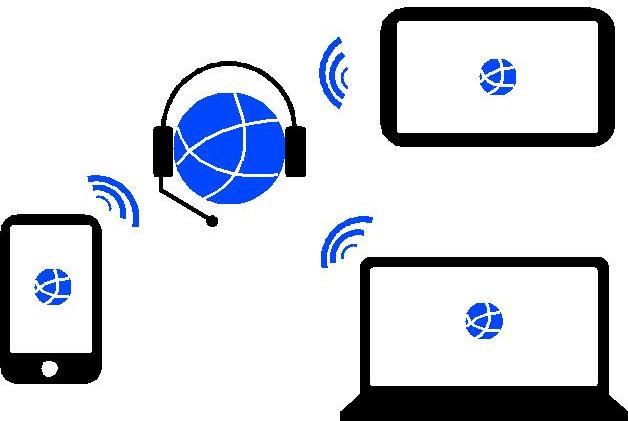
\includegraphics[width=0.5\textwidth]{img/plattformUnabhaengigkeit.jpg}
		\label{plattformUnabhaengigkeit}
	\end{figure}
	
	Durch den offenen Standard ``WebRTC''\footnote{W3C, WebRCT 1.0: Real-time Communication Between Browsers, Draft (Stand: 10.09.13). \hyperlink{http://www.w3.org/TR/webrtc/}{http://www.w3.org/TR/webrtc/}, [Abruf am 21.11.13]}
	 ist die Applikation auf jedem modernen Gerät benutzbar, das den Standard umsetzt und genug Leistung für Audio- und Videokommunikation bereitstellt.
	
	Durch die einfache Benutzung ist die Applikation auch für nicht versierte Benutzer zugänglich.
	
	Das integrierte Kontaktmanagement kann mit verschiedenen Importformaten umgehen und einfach um weitere Quellen erweitert werden. Dazu gibt es eine Adressbuchschnittstelle.
	
	Die Applikation kann um beliebige Signallingchannel erweitert werden. Somit ist es unter Anderem möglich, die Applikation um signalling über SIP oder XMPP zu erweitern. Dazu gibt es eine Channelschnittstelle.
	
		